\documentclass[12pt,a4paper]{article}

% ── Geometry & spacing ──────────────────────────────────────
\usepackage[margin=2.5cm]{geometry}
\setlength{\headheight}{14.5pt}
\addtolength{\topmargin}{-2.5pt}
\setlength{\parindent}{1.25em}
\setlength{\parskip}{0pt}

% ── Encoding & language ─────────────────────────────────────
\usepackage[T1]{fontenc}
\usepackage[utf8]{inputenc}
% Swap the two lines below to switch language:
% \usepackage[english]{babel}       
\usepackage[indonesian]{babel}     % Bahasa Indonesia

% ── Font ────────────────────────────────────────────────────
\usepackage{lmodern}

% ── Math ────────────────────────────────────────────────────
\usepackage{amsmath, amssymb, amsthm}
\usepackage{mathtools}

% ── Graphics & figures ──────────────────────────────────────
\usepackage{graphicx}
\usepackage{float}
\usepackage{caption}
\usepackage{subcaption}
\graphicspath{{doc/}}

% ── Tables ──────────────────────────────────────────────────
\usepackage{booktabs}
\usepackage{array}
\usepackage{longtable}

% ── Lists ───────────────────────────────────────────────────
\usepackage{enumitem}

% ── Code listings ───────────────────────────────────────────
\usepackage{listings}
\usepackage{xcolor}

\definecolor{codebg}{RGB}{245,245,245}
\definecolor{codeframe}{RGB}{200,200,200}
\definecolor{codekw}{RGB}{0,0,180}
\definecolor{codecomment}{RGB}{60,128,49}
\definecolor{codestring}{RGB}{163,21,21}

\lstdefinestyle{default}{
  backgroundcolor=\color{codebg},
  basicstyle=\ttfamily\small,
  breaklines=true,
  breakatwhitespace=false,
  tabsize=2,
  showstringspaces=false,
  frame=single,
  rulecolor=\color{codeframe},
  numbers=left,
  numberstyle=\tiny\color{gray},
  numbersep=8pt,
  xleftmargin=2.5em,
  framexleftmargin=2em,
  keywordstyle=\color{codekw}\bfseries,
  commentstyle=\color{codecomment}\itshape,
  stringstyle=\color{codestring},
}
\lstdefinestyle{go}{style=default, language=Python}    % closest builtin
\lstdefinestyle{python}{style=default, language=Python}
\lstdefinestyle{java}{style=default, language=Java}
\lstdefinestyle{cpp}{style=default, language=C++}
\lstdefinestyle{bash}{style=default, language=bash}

\lstset{style=default}   % global default

% ── Boxes (for tips / callouts) ──────────────────────────────
\usepackage{tcolorbox}
\tcbuselibrary{listings, skins, breakable}

\newtcolorbox{infobox}[1][Note]{
  colback=blue!5!white, colframe=blue!50!black,
  fonttitle=\bfseries, title=#1,
  breakable
}
\newtcolorbox{warnbox}[1][Warning]{
  colback=orange!10!white, colframe=orange!80!black,
  fonttitle=\bfseries, title=#1,
  breakable
}

\usepackage{hyperref}
\usepackage{xurl}
\hypersetup{colorlinks=true, linkcolor=black, urlcolor=blue, citecolor=black}

\usepackage{siunitx}

\usepackage{fancyhdr}
\pagestyle{fancy}
\fancyhf{}
\lhead{\CourseCode{} -- \CourseName}
\rhead{\thepage}

% ── First-line indent on all sections ───────────────────────
\usepackage{indentfirst}

\newcommand{\CourseCode}{IF2224}
\newcommand{\CourseName}{Teori Bahasa Formal dan Otomata}
\newcommand{\AssignmentTitle}{Laporan Tugas Besar}
\newcommand{\AssignmentSubtitle}{Milestone 3: Semantic Analysis}
\newcommand{\Semester}{Semester II / 2025--2026}

% Team / group
\newcommand{\GroupName}{GTFOTBFO (HBB)}
\newcommand{\MemberA}{Nathanael Imandatua Manurung - 13524021}
\newcommand{\MemberB}{Nicholas Wise Saragih Sumbayak - 13524037}
\newcommand{\MemberC}{Kurt Mikhael Purba - 13524065}
\newcommand{\MemberD}{Rava Khoman Tuah Saragih - 13524107}


% Institution
\newcommand{\Lab}{Laboratorium Ilmu dan Rekayasa Komputasi}
\newcommand{\Program}{Teknik Informatika}
\newcommand{\Faculty}{Sekolah Teknik Elektro dan Informatika}
\newcommand{\University}{Institut Teknologi Bandung}

% Repository link (used in Appendix)
\newcommand{\RepoURL}{https://github.com/nicholaswisee/HBB-Tubes-IF2224-2026}
\newcommand{\DeployURL}{https://your-deployment-url.example.com}
\newcommand{\DFAURL}{https://drive.google.com/file/d/1XT-esS_K76ImoWZUwJKy43QvJW_NdP0a/view}

\begin{document}

\begin{titlepage}
  \begin{center}
    \vspace*{1cm}
    {\Huge \textbf{\AssignmentTitle}}\\[0.4cm]
    {\Large \textsc{\CourseCode{} \CourseName}}\\[0.2cm]
    {\large \textsc{\AssignmentSubtitle}}\\[0.2cm]
    {\large \textsc{\Semester}}\\[2cm]

    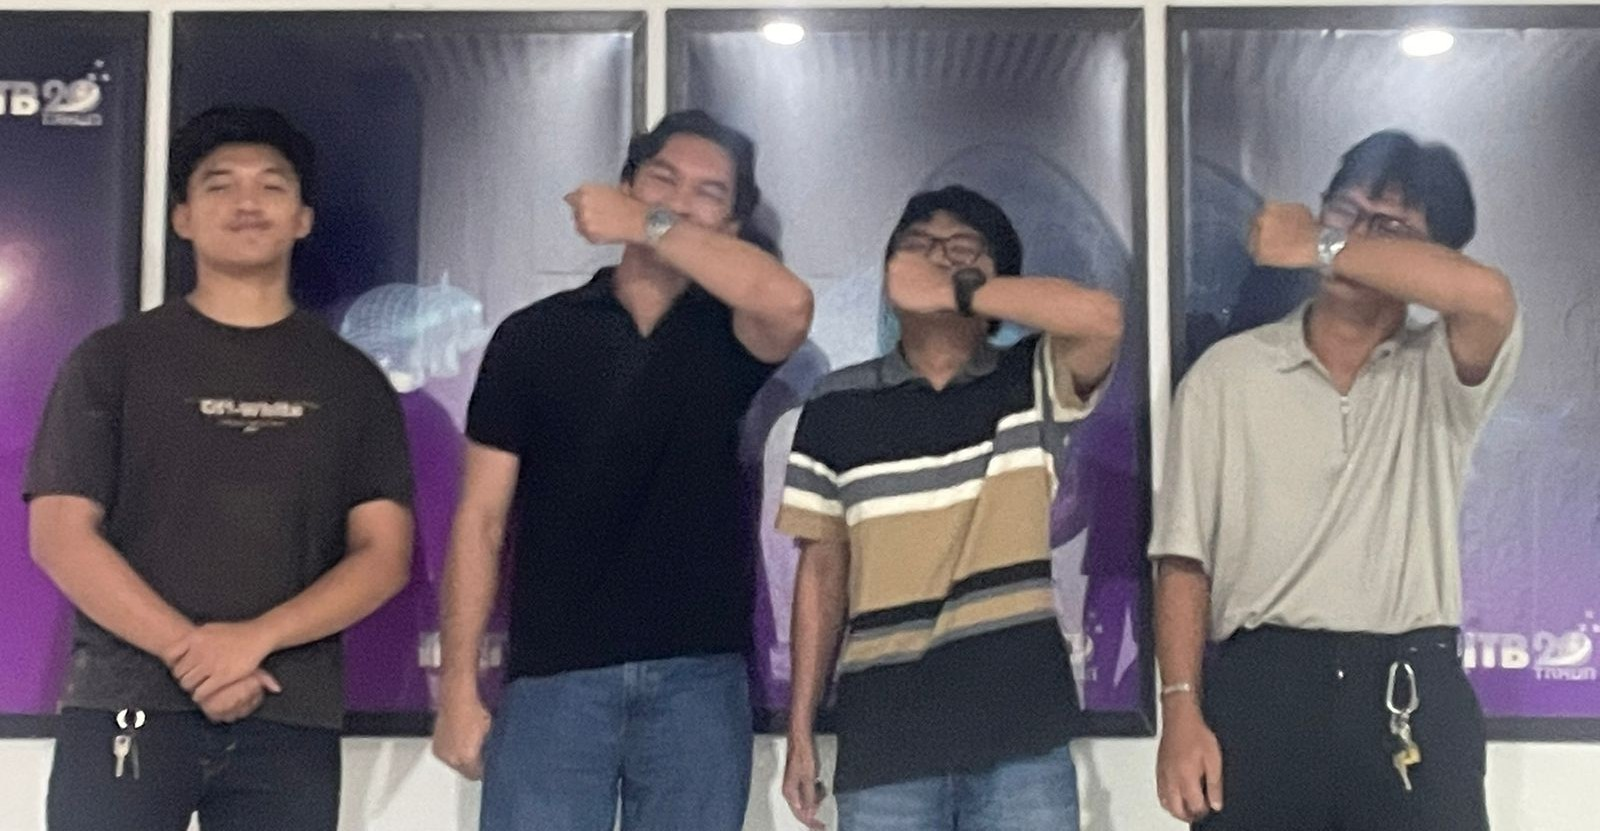
\includegraphics[height=8cm]{nael.jpeg}\\[2cm]

    {\large \textbf{Disusun oleh:}}\\[0.3cm]
    {\large
      \textbf{\GroupName}\\[0.25cm]
      \MemberA\\
      \MemberB\\
      \MemberC\\
      \MemberD\\
    }

    \vfill

    {\large \textsc{\Lab}}\\[0.15cm]
    {\large \textsc{Program Studi \Program}}\\[0.15cm]
    {\large \textsc{\Faculty}}\\[0.15cm]
    {\large \textsc{\University}}\\
  \end{center}
\end{titlepage}

\tableofcontents
\newpage

\section{Pendahuluan}

Pada tahap sebelumnya, telah berhasil dibangun sebuah \textit{syntax analyzer}
(parser) yang mampu memeriksa urutan token dari \textit{lexical analyzer} dan
membangun \textit{Parse Tree} sesuai dengan aturan \textit{grammar} bahasa
Arion. Meskipun parser telah berfungsi dengan baik dalam memverifikasi struktur
sintaks program, parser belum mampu memastikan apakah program tersebut memiliki
makna (\textit{meaning}) yang benar sesuai dengan aturan semantik bahasa Arion.

Proses transformasi kode sumber menjadi program yang dapat dijalankan melibatkan
beberapa tahap berurutan. Setelah analisis sintaktik selesai, tahap berikutnya
adalah analisis semantik (\textit{semantic analysis}). Pada tahap ini,
\textit{semantic analyzer} menerima \textit{Parse Tree} dari parser dan
melakukan pemeriksaan makna program, seperti kecocokan tipe data (\textit{type
checking}), pengelolaan \textit{scope}, dan validasi penggunaan
\textit{identifier} yang telah dideklarasikan. Hasil dari tahap ini adalah
\textit{Decorated Abstract Syntax Tree} (Decorated AST) yang telah dianotasi
dengan informasi tipe data dan referensi ke \textit{symbol table}.

\begin{figure}[H]
\centering
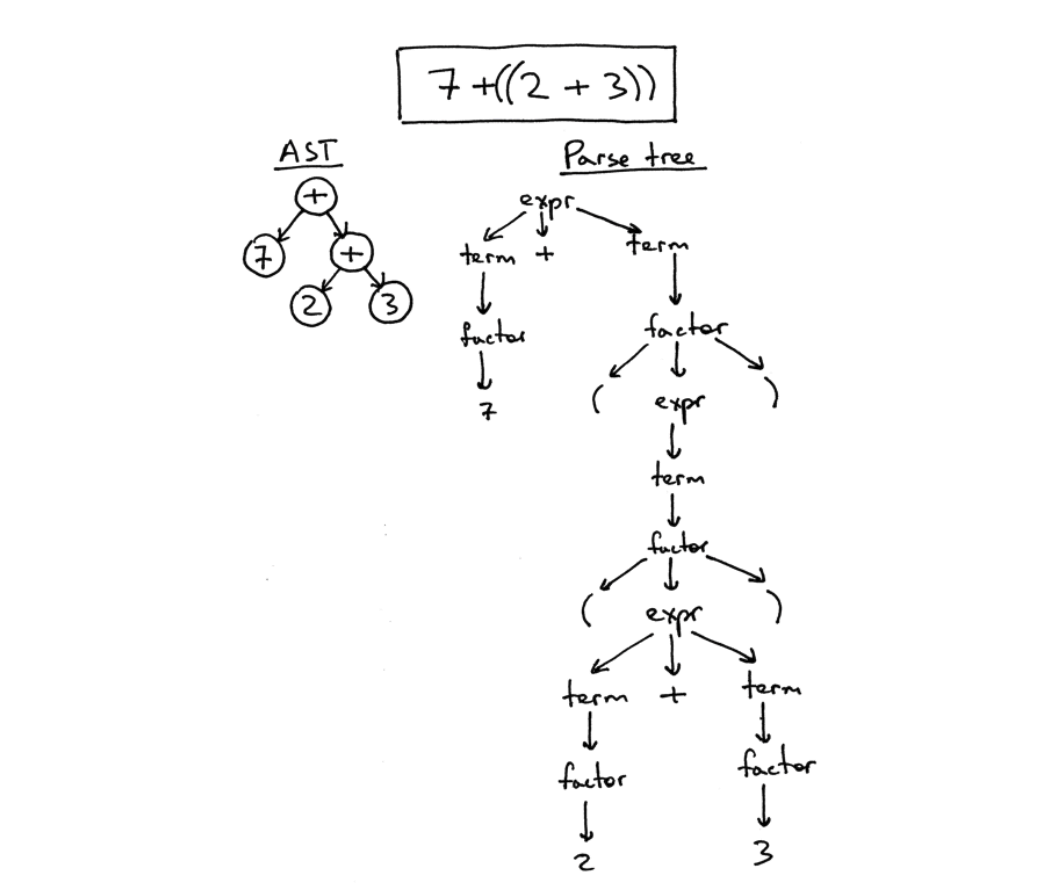
\includegraphics[height=10cm]{parse-ast.png}
\caption{Tahapan transformasi dari Parse Tree ke Decorated AST}
\caption*{Sumber: Spesifikasi Milestone 3 IF2224}
\end{figure}

\textit{Abstract Syntax Tree} (AST) adalah representasi ringkas dari
\textit{Parse Tree} yang hanya menyimpan informasi esensial untuk tahap analisis
semantik dan selanjutnya. Berbeda dengan \textit{Parse Tree} yang memuat semua
detail sintaksis (termasuk tanda kurung, kata kunci, dan tanda baca), AST
menghilangkan informasi yang sudah tidak diperlukan dan berfokus pada hubungan
semantik antar operator dan operand. \textit{Decorated AST} merupakan AST yang
telah dianotasi dengan informasi tambahan seperti tipe data, referensi
\textit{symbol table}, dan tingkatan \textit{scope}.

\subsection{Latar Belakang}

Proses kompilasi suatu bahasa pemrograman terdiri atas beberapa tahap yang
saling berkaitan, dimulai dari analisis leksikal (\textit{lexical analysis}),
analisis sintaktik (\textit{syntax analysis}), analisis semantik
(\textit{semantic analysis}), hingga pembangkitan kode (\textit{code
generation}). Setelah parser berhasil memverifikasi struktur sintaks program dan
membangun \textit{Parse Tree}, tahap analisis semantik menjadi penting untuk
memastikan bahwa program tidak hanya benar secara sintaksis, tetapi juga
memiliki makna yang valid.

Pada tugas besar mata kuliah IF2224 Teori Bahasa Formal dan Otomata, mahasiswa
diminta untuk membangun sebuah \textit{compiler} sederhana untuk bahasa
pemrograman Arion, yaitu bahasa bertipe Pascal. Milestone ketiga ini berfokus
pada pembangunan \textit{semantic analyzer} yang mampu mengkonversi
\textit{Parse Tree} menjadi \textit{AST}, melakukan pengecekan semantik
menggunakan \textit{Attributed Grammar}, mengelola \textit{symbol table} untuk
menyimpan informasi \textit{identifier}, dan menghasilkan \textit{Decorated AST}
yang teranotasi.

\subsection{Rumusan Masalah}

Bagaimana merancang dan mengimplementasikan sebuah \textit{semantic analyzer} berbasis \textit{Attributed Grammar} dan \textit{Visitor Pattern} yang mampu:

\begin{enumerate}[label=\arabic*.]
  \item Mengkonversi \textit{Parse Tree} menjadi \textit{Abstract Syntax Tree} (AST) yang ringkas.
  \item Membangun dan mengelola \textit{symbol table} (\texttt{tab}, \texttt{btab}, \texttt{atab}) untuk menyimpan informasi \textit{identifier}.
  \item Melakukan pengecekan tipe data (\textit{type checking}) dan kompatibilitas antar tipe.
  \item Mengelola \textit{scope} dan memastikan setiap \textit{identifier} telah dideklarasikan sebelum digunakan.
  \item Menghasilkan \textit{Decorated AST} yang teranotasi dengan informasi semantik.
\end{enumerate}

\subsection{Gambaran Umum Sistem}

Sistem yang dibangun merupakan sebuah \textit{semantic analyzer} untuk bahasa Arion yang diimplementasikan dalam bahasa C++20. \textit{Semantic analyzer} ini menerima \textit{Parse Tree} dari tahap \textit{syntax analysis}, mengkonversinya menjadi \textit{AST}, melakukan penelusuran \textit{depth-first search} (DFS) menggunakan \textit{visitor functions}, mengelola \textit{symbol table}, melakukan \textit{type checking}, dan menghasilkan \textit{Decorated AST} beserta informasi \textit{symbol table} sebagai keluaran.

Sistem terdiri atas beberapa komponen utama:

\begin{itemize}
  \item \textbf{ParseTreeToAST}: Konverter dari \textit{Parse Tree} ke \textit{AST} menggunakan \textit{Syntax-Directed Translation}.
  \item \textbf{ASTNode}: Struktur data \textit{node} pada \textit{AST} yang merepresentasikan hubungan semantik antar operator dan operand.
  \item \textbf{SymbolTableManager}: Pengelola \textit{symbol table} (\texttt{tab}, \texttt{btab}, \texttt{atab}) untuk penyimpanan dan pencarian \textit{identifier}.
  \item \textbf{SemanticAnalyzer}: Mesin analisis semantik menggunakan \textit{Visitor Pattern} untuk melakukan \textit{type checking} dan \textit{scope resolution}.
  \item \textbf{TypeSystem}: Sistem tipe data dan aturan kompatibilitas tipe.
\end{itemize}

\subsection{Spesifikasi Umum}

\begin{enumerate}[label=\arabic*.]
  \item Menggunakan \textit{Attributed Grammar} dengan \textit{semantic actions} pada aturan produksi grammar.
  \item Mengimplementasikan \textit{symbol table} dengan struktur \texttt{tab}, \texttt{btab}, dan \texttt{atab} sesuai spesifikasi.
  \item Mendukung \textit{scope resolution} dengan mekanisme \textit{push} dan \textit{pop} pada \textit{symbol table}.
  \item Melakukan \textit{type checking} dan \textit{type inference} sesuai aturan kompatibilitas tipe bahasa Arion.
  \item Menghasilkan \textit{Decorated AST} yang teranotasi dengan informasi tipe data dan referensi \textit{symbol table}.
  \item Melaporkan kesalahan semantik (\textit{semantic error}) dengan pesan yang informatif dan akurat.
\end{enumerate}


\section{Dasar Teori}

\subsection{Pendefinisian Bahasa Pemrograman}
Bahasa Pemrograman adalah cara manusia untuk dapat memberikan perintah
(\textit{instruction}) kepada sebuah komputer. Setiap bahasa pemrograman
memiliki kata kunci dan aturannya masing-masing serta makna dari kata-kata itu
yang disebut sintaks(\textit{syntax}) dan semantik (\textit{semantics}).
Input yang terdapat kesalahan pada tingkat sintaks berarti input tersebut tidak
valid untuk bahasa pemrograman tersebut, sedangkan kesalahan pada tingkat
semantik umumnya berbentuk kesalahan logika atau ketidakcocokan tipe data.

\subsubsection{Hierarki Bahasa Pemrograman}
Berdasarkan tingkat abstraksinya, bahasa pemrograman diklasifikasikan menjadi dua kategori utama:
\begin{itemize}
\item \textbf{\textit{Low-Level Language} (Bahasa Tingkat Rendah)}: Bahasa yang instruksinya mendekati arsitektur perangkat keras dan bahasa mesin (biner 0 dan 1). Contohnya adalah \textit{Assembly}, yang memerlukan \textit{Assembler} untuk menerjemahkan kode menjadi instruksi yang dapat dipahami CPU.
\item \textbf{\textit{High-Level Language} (Bahasa Tingkat Tinggi)}: Bahasa yang dirancang agar lebih mudah dibaca dan dipahami oleh manusia karena menggunakan kosakata yang menyerupai bahasa natural. Semakin tinggi tingkat bahasa tersebut, semakin banyak tahapan pemrosesan yang diperlukan untuk mengubahnya menjadi kode mesin. Contoh bahasa tingkat tinggi antara lain Pascal, C++, Python, dan Java.
\end{itemize}

\subsubsection{\textit{Compiler} dan \textit{Interpreter} }
Untuk menjalankan kode sumber yang ditulis dalam bahasa tingkat tinggi,
diperlukan sebuah perangkat lunak penerjemah yang mengubah kode tersebut menjadi
format yang dapat dieksekusi oleh mesin. Secara umum, terdapat dua mekanisme
utama untuk mengubah bahasa tingkat tinggi ke bahasa mesin:

\begin{enumerate}
\item \textbf{\textit{Compiler} (Kompilator)}:
\textit{Compiler} adalah program yang menerjemahkan seluruh \textit{source code}
secara utuh menjadi kode mesin (biasanya dalam bentuk \textit{Object File})
sebelum program dijalankan. Proses kompilasi pada \textit{compiler} umumnya
terdiri dari empat tahapan utama: \textit{Lexical Analysis}, \textit{Syntax
Analysis}, \textit{Semantic Analysis}, dan \textit{Intermediate Code
Generation}. Karakteristik utama \textit{compiler} adalah jika terdeteksi adanya
kesalahan (\textit{error}) di dalam \textit{source code}, maka seluruh proses
kompilasi akan gagal dan program tidak dapat dijalankan.

\item \textbf{\textit{Interpreter}}:
Berbeda dengan \textit{compiler}, \textit{interpreter} memproses kode sumber
baris demi baris secara langsung. \textit{Interpreter} membaca,
menerjemahkan, dan langsung mengeksekusi kode mesin tersebut baris demi baris.
Hal ini memungkinkan program tetap berjalan normal hingga baris sebelum
ditemukannya kesalahan; misalnya, jika terdapat \textit{error} pada baris ke-10,
baris 1 sampai 9 akan tetap berhasil dieksekusi. Meskipun mekanisme eksekusinya
berbeda, \textit{interpreter} sebenarnya memiliki tahapan pemrosesan internal
yang serupa dengan \textit{compiler}.

\end{enumerate}

\subsection{Teori Kompilator (\textit{Compiler Theory})}

Proses kompilasi adalah urutan dari berbagai fase (\textit{phases}) yang bekerja secara berurutan. Setiap fase mengambil input dari tahap sebelumnya, memprosesnya, dan memberikan output yang akan digunakan sebagai input untuk fase berikutnya. Secara umum, arsitektur sebuah kompilator terdiri dari fase-fase berikut:

\begin{enumerate}
    \item \textbf{\textit{Lexical Analysis}}: Fase pertama yang bekerja sebagai
        pemindai teks (\textit{text scanner}) pada kode sumber.
    \item \textbf{\textit{Syntax Analysis} (\textit{Parsing})}: Mengambil
        \textit{token} yang dihasilkan oleh \textit{lexical analysis} dan
        membangun pohon sintaksis (\textit{parse tree}).
    \item \textbf{\textit{Semantic Analysis}}: Memeriksa apakah pohon sintaksis
        yang dibangun mengikuti aturan semantik bahasa, seperti kecocokan
        operasi tipe data dan memastikan \textit{identifier} telah
        dideklarasikan sebelum digunakan. Fase ini menghasilkan keluaran berupa
        pohon sintaksis yang dianotasi (\textit{Decorated AST}).
    \item \textbf{\textit{Intermediate Code Generation}}: Menghasilkan
        representasi kode perantara untuk mesin abstrak.
    \item \textbf{\textit{Code Optimization}}: Mengoptimalkan kode perantara
        dengan menghapus baris kode yang tidak perlu dan mengatur ulang urutan
        instruksi.
    \item \textbf{\textit{Target Code Generation}}: Merupakan fase sintesis
    akhir (\textit{back-end}) yang menggunakan representasi kode perantara dan
    tabel simbol untuk menghasilkan program target atau bahasa mesin.
\end{enumerate}

\subsubsection{Analisis Semantik (\textit{Semantic Analysis})}

Sebagai fokus utama pada \textit{milestone} ini, Analisis Semantik atau
\textit{semantic analyzer} adalah tahapan atau fase ketiga dari sebuah kompilator. Fase ini bertugas untuk memeriksa makna (\textit{meaning}) dari program yang telah berhasil melewati tahap analisis sintaktik. \textit{Semantic analyzer} menerima \textit{Parse Tree} dari parser dan melakukan berbagai pemeriksaan semantik, antara lain:

\begin{itemize}
    \item \textbf{\textit{Type Checking}}: Memastikan operator dan operand memiliki tipe yang kompatibel. Contohnya: tidak menjumlahkan \textit{string} dengan \textit{integer}, atau memastikan kondisi pada \textit{if-statement} bertipe \textit{Boolean}.
    \item \textbf{\textit{Symbol Table Management}}: Memastikan setiap \textit{identifier} (variabel, fungsi, prosedur) telah dideklarasikan sebelum digunakan dan tidak dideklarasikan ulang dalam \textit{scope} yang sama.
    \item \textbf{\textit{Scope Resolution}}: Menentukan validitas akses variabel berdasarkan hierarki blok kode (\textit{scope} global vs \textit{scope} lokal).
    \item \textbf{\textit{Control Flow Validation}}: Memastikan struktur alur kontrol yang logis, seperti memastikan instruksi \texttt{break}/\texttt{continue} hanya berada dalam \textit{loop}, atau fungsi memiliki \texttt{return} pada semua cabang kontrol.
\end{itemize}

\textit{Semantic analyzer} akan melakukan anotasi terhadap \textit{Parse Tree} untuk menghasilkan \textit{Decorated Abstract Syntax Tree} (Decorated AST). Anotasi berupa penambahan informasi seperti tipe data dan referensi \textit{identifier} ke \textit{symbol table}.

\subsection{Teori Bahasa Formal dan Otomata}

Setelah tahap analisis sintaktik menggunakan \textit{Context-Free Grammar} (CFG) untuk memeriksa struktur program, tahap analisis semantik menggunakan konsep \textit{Attributed Grammar} sebagai dasar untuk melakukan pengecekan makna program.

\subsubsection{Abstract Syntax Tree (AST)}

\textit{Abstract Syntax Tree} (AST) pada dasarnya adalah bentuk ringkas dari \textit{Parse Tree}, dimana hanya informasi yang diperlukan untuk tahapan selanjutnya yang disimpan dan informasi yang sudah tidak lagi diperlukan untuk tahap analisis dibuang. Struktur dasar sebuah \textit{Parse Tree} didasarkan pada aturan \textit{Grammar} untuk melakukan pengecekan \textit{syntax}. Namun pada tahap \textit{Semantic Analysis} dan selanjutnya, konteks sintaksis tersebut tidak lagi diperlukan.

Pada \textit{AST}, fokus berpindah menuju aturan semantik, yaitu mengenai hubungan antar operator dan operand. Aturan tersebut menjadi penting untuk pengecekan semantik dan tahapan selanjutnya. Sebagai ilustrasi, untuk potongan kode:

\begin{lstlisting}
while (i > 0) {
    x = x + z * 5;
}
\end{lstlisting}

\textit{Parse Tree} akan memuat semua detail sintaksis (termasuk tanda kurung, kurung kurawal, dan semicolon), sedangkan \textit{AST} akan menyederhanakan representasi tersebut menjadi struktur yang hanya memuat informasi esensial: sebuah \textit{node} \texttt{While} dengan kondisi \texttt{i > 0} dan tubuh berupa penugasan \texttt{x = x + (z * 5)}.

\subsubsection{Decorated Abstract Syntax Tree (Decorated AST)}

\textit{Semantic Analysis} akan melakukan anotasi terhadap \textit{AST} hasil konversi dari \textit{Parse Tree} untuk menghasilkan sebuah \textit{Decorated AST}. Anotasi yang dilakukan bertujuan memberikan konteks untuk pengecekan semantik, seperti penambahan \textit{symbol table}, tipe data, penambahan \textit{reserved keywords}, pelacakan \textit{identifier}, penanda tingkatan \textit{scope}, dan sebagainya.

Implementasi \textit{Decorated AST} memang beragam, namun dalam tugas ini, berbasis tiga \textit{symbol table} utama: \texttt{tab}, \texttt{btab}, dan \texttt{atab}. Jadi \textit{Decorated AST} merupakan hasil dari proses pengecekan semantik pada \textit{Semantic Analysis}.

Beberapa istilah penting yang perlu dipahami:

\begin{itemize}
    \item \textbf{\textit{Attributed Grammar}}: Grammar yang dilengkapi dengan atribut dan aturan semantik. Setiap aturan produksi memiliki \textit{semantic actions} yang dieksekusi saat aturan tersebut diterapkan.
    \item \textbf{\textit{Symbol Table}}: Struktur data yang minimal menyimpan informasi nama \textit{identifier}, tipe datanya, dan \textit{scope}-nya. \textit{Symbol table} menggunakan struktur data \textit{stack} untuk mengelola \textit{scope}.
    \item \textbf{\textit{Visitor} / \textit{Visit Functions}}: Untuk setiap jenis \textit{node} akan memiliki fungsi \texttt{visit\_\textless{}node\textgreater{}} yang akan memanggil \textit{visit} pada \textit{child}-nya, mengakses atau memperbarui \textit{symbol table}, menghitung atribut/tipe semantik, dan menambahkan anotasi pada \textit{node}.
\end{itemize}

\subsubsection{Symbol Table}

\textit{Symbol Table} adalah struktur data yang digunakan oleh \textit{semantic analyzer} untuk menyimpan informasi tentang \textit{identifier} yang ditemui dalam program. Informasi yang disimpan meliputi nama \textit{identifier}, jenis objek (konstanta, variabel, tipe, prosedur, fungsi), tipe data, tingkat \textit{scope} (\textit{lexical level}), dan alamat memori.

Dalam implementasi bahasa Arion, terdapat tiga jenis \textit{symbol table}:

\begin{enumerate}
    \item \textbf{\texttt{tab} (Identifier Table)}: Menyimpan informasi mengenai \textit{identifier} termasuk konstanta, variabel, prosedur, atau fungsi. Setiap entri memiliki atribut: \texttt{id} (nama), \texttt{link} (pointer ke \textit{identifier} sebelumnya dalam \textit{scope} yang sama), \texttt{obj} (jenis objek), \texttt{type} (tipe data), \texttt{ref} (pointer ke tabel lain jika tipe komposit), \texttt{nrm} (penanda variabel normal atau \textit{var parameter}), \texttt{lev} (tingkat \textit{lexical level}), dan \texttt{adr} (alamat/offset).

    \item \textbf{\texttt{btab} (Block Table)}: Menyimpan informasi blok prosedur dan definisi tipe rekord. Setiap entri memiliki atribut: \texttt{last} (pointer ke \textit{identifier} terakhir), \texttt{lpar} (pointer ke parameter terakhir), \texttt{psze} (total ukuran parameter), dan \texttt{vsze} (total ukuran variabel lokal).

    \item \textbf{\texttt{atab} (Array Table)}: Menyimpan informasi \textit{array} seperti tipe \textit{index}, batasan \textit{index}, tipe elemen, dan ukuran \textit{array}. Setiap entri memiliki atribut: \texttt{xtyp} (tipe \textit{index}), \texttt{etyp} (tipe elemen), \texttt{eref} (pointer ke detail tipe elemen), \texttt{low} (batas bawah), \texttt{high} (batas atas), \texttt{elsz} (ukuran satu elemen), dan \texttt{size} (total ukuran \textit{array}).
\end{enumerate}

\subsubsection{Type Checking dan Type Compatibility}

\textit{Type Checking} adalah proses memastikan bahwa setiap operasi dalam program menggunakan tipe data yang kompatibel. Aturan kompatibilitas tipe (\textit{Type Compatibility Rules}) menentukan bagaimana tipe dapat digunakan dalam ekspresi, \textit{statement} (misalnya penugasan), dan lainnya.

Dalam bahasa Arion, terdapat beberapa aturan dasar kompatibilitas tipe:

\begin{itemize}
    \item \textbf{Compatible Types}: Dua tipe dikatakan \textit{compatible} jika memiliki tipe yang sama, atau salah satu adalah \textit{subrange} dari yang lain.
    \item \textbf{Assignment Compatible}: Tipe \texttt{T2} adalah \textit{assignment-compatible} dengan \texttt{T1} jika \texttt{T1} adalah \texttt{Real} dan \texttt{T2} adalah \texttt{Integer}, atau keduanya \textit{compatible} dengan nilai \texttt{T2} merupakan \textit{subset} dari nilai \texttt{T1}.
    \item \textbf{Operator Rules}: Operator aritmatika (\texttt{+}, \texttt{-}, \texttt{*}, \texttt{/}, \texttt{div}, \texttt{mod}) memerlukan operand numerik (\texttt{Integer} atau \texttt{Real}). Operator relasional (\texttt{=}, \texttt{<>}, \texttt{<}, \texttt{<=}, \texttt{>}, \texttt{>=}) memerlukan operand yang dapat dibandingkan. Operator logika (\texttt{and}, \texttt{or}, \texttt{not}) memerlukan operand \texttt{Boolean}.
\end{itemize}

\section{Perancangan Semantic Analyzer}

Perancangan \textit{semantic analyzer} untuk bahasa Arion didasarkan pada konsep \textit{Attributed Grammar} dengan pendekatan \textit{Syntax-Directed Translation} untuk mengkonversi \textit{Parse Tree} menjadi \textit{AST}, serta \textit{Visitor Pattern} untuk melakukan penelusuran \textit{AST} dan pengecekan semantik. Pada bagian ini, dijelaskan rancangan konversi \textit{Parse Tree} ke \textit{AST}, perancangan \textit{symbol table}, perancangan \textit{visitor functions}, dan alur kerja program.

\subsection{Konversi Parse Tree ke AST}

Konversi dari \textit{Parse Tree} ke \textit{AST} dilakukan menggunakan pendekatan \textit{Syntax-Directed Translation} (SDT). Pada setiap aturan produksi \textit{grammar}, disisipkan \textit{semantic actions} yang menentukan bagaimana \textit{node-node} dari \textit{Parse Tree} dikonversi menjadi \textit{node-node} \textit{AST}.

\textit{Semantic actions} berfungsi untuk mengevaluasi nilai atribut dari masing-masing \textit{node}. Proses konversi dilakukan dengan:
\begin{enumerate}
    \item Membentuk \textit{node} baru untuk \textit{AST} (seperti \texttt{AssignNode}, \texttt{BinOpNode}) yang merepresentasikan hubungan semantik antar operator dan operand.
    \item Menghilangkan informasi sintaksis yang sudah tidak diperlukan untuk tahap analisis (seperti tanda kurung berlebih, kata kunci terminal \texttt{BEGIN}, \texttt{END}, dan \texttt{SEMICOLON}).
    \item Menggabungkan potongan \textit{node} dari bawah ke atas dengan \textit{node} level bawah akan diserahkan ke \textit{node} induknya untuk dirakit menjadi satu kesatuan \textit{AST} yang utuh.
\end{enumerate}

Berikut adalah contoh aturan konversi untuk beberapa konstruksi bahasa:

\begin{table}[H]
\centering
\caption{Aturan Konversi Parse Tree ke AST}
\begin{tabular}{|l|l|}
\hline
\textbf{Production Rule} & \textbf{Semantic Action} \\
\hline
$\langle\text{assignment}\rangle \rightarrow \text{ID} \; \texttt{becomes} \; \langle\text{expr}\rangle$ & assign.node = \texttt{AssignNode}(ID.name, expr.node) \\
\hline
$\langle\text{expr}\rangle \rightarrow \langle\text{expr}\rangle \; \texttt{+} \; \langle\text{term}\rangle$ & expr.node = \texttt{BinOpNode}('+', expr.node, term.node) \\
\hline
$\langle\text{factor}\rangle \rightarrow \text{INTCON}$ & factor.node = \texttt{LiteralNode}(INTCON.value, Integer) \\
\hline
$\langle\text{factor}\rangle \rightarrow \text{ID}$ & factor.node = \texttt{VarNode}(ID.name) \\
\hline
\end{tabular}
\end{table}

\subsection{Perancangan Symbol Table}

\textit{Symbol table} dirancang dengan tiga struktur data utama sesuai spesifikasi:

\begin{itemize}
    \item \textbf{\texttt{tab}}: \textit{Vector} dari \texttt{TabEntry} untuk menyimpan informasi \textit{identifier}. Indeks 0--32 dicadangkan untuk \textit{reserved words} dan tipe predefined. \textit{Identifier} yang didefinisikan pengguna dimulai dari indeks 33.
    \item \textbf{\texttt{btab}}: \textit{Vector} dari \texttt{BTabEntry} untuk menyimpan informasi blok. Indeks 0 merupakan blok global (program utama).
    \item \textbf{\texttt{atab}}: \textit{Vector} dari \texttt{ATabEntry} untuk menyimpan informasi \textit{array}.
\end{itemize}

Pengelolaan \textit{scope} dilakukan dengan mekanisme \textit{display} yang menyimpan indeks \texttt{btab} untuk setiap tingkat \textit{lexical level}. Saat memasuki blok baru (fungsi, prosedur, atau rekord), dilakukan \textit{push} pada \textit{symbol table}, dan saat keluar dari blok, dilakukan \textit{pop}.

\subsection{Perancangan Semantic Visitor}

\textit{Semantic analyzer} dirancang menggunakan \textit{Visitor Pattern} dengan fungsi-fungsi \texttt{visit} untuk setiap jenis \textit{node} \textit{AST}:

\begin{itemize}
    \item \textbf{Visit Declarations}: Melakukan registrasi \textit{identifier} ke \textit{symbol table} (\texttt{tab}) setiap kali ditemukan deklarasi konstanta, variabel, tipe, prosedur, atau fungsi.
    \item \textbf{Visit Statements}: Melakukan \textit{lookup} pada \textit{symbol table} untuk memastikan \textit{identifier} telah dideklarasikan, serta melakukan \textit{type checking} pada setiap operasi dan penugasan.
    \item \textbf{Visit Expressions}: Melakukan inferensi tipe data hasil dari setiap operasi pada \textit{node} (misalnya, operasi dua operand \texttt{Integer} menghasilkan tipe \texttt{Integer}).
\end{itemize}

Setiap fungsi \texttt{visit} akan melakukan anotasi pada \textit{node} dengan informasi tambahan seperti tipe data akhir dari ekspresi, referensi atau indeks yang mengarah pada entri yang tepat di \textit{symbol table}, dan tingkatan \textit{lexical level} atau \textit{scope} tempat \textit{node} tersebut berada.

\subsection{Perancangan Type System}

\textit{Type system} dirancang untuk mengelola tipe data dan aturan kompatibilitas dalam bahasa Arion. Tipe dasar yang didukung meliputi:

\begin{itemize}
    \item \texttt{Integer} untuk bilangan bulat
    \item \texttt{Real} untuk bilangan riil
    \item \texttt{Char} untuk karakter tunggal
    \item \texttt{Boolean} untuk nilai logika
    \item \texttt{String} untuk rangkaian karakter
\end{itemize}

Tipe \textit{structured} yang didukung meliputi \textit{array} dan \textit{record}. Aturan kompatibilitas tipe mencakup:
\begin{itemize}
    \item Dua tipe \textit{compatible} jika memiliki tipe yang sama.
    \item \texttt{Real} dapat menerima \texttt{Integer} dalam penugasan (\textit{assignment-compatible}).
    \item Operator aritmatika menghasilkan \texttt{Real} jika salah satu operand adalah \texttt{Real}, dan \texttt{Integer} jika keduanya \texttt{Integer}.
    \item Operator relasional selalu menghasilkan \texttt{Boolean}.
\end{itemize}

\subsection{Strategi Penanganan Kesalahan}

\textit{Semantic analyzer} dirancang untuk menangani berbagai jenis kesalahan semantik:

\begin{itemize}
    \item \textbf{Undeclared Identifier}: \textit{Identifier} yang digunakan tetapi belum dideklarasikan dalam \textit{scope} yang berlaku.
    \item \textbf{Redeclaration}: \textit{Identifier} yang dideklarasikan lebih dari satu kali dalam \textit{scope} yang sama.
    \item \textbf{Type Mismatch}: Penugasan atau operasi antara dua tipe yang tidak \textit{compatible}.
    \item \textbf{Invalid Operation}: Penggunaan operator pada tipe yang tidak didukung (misalnya aritmatika pada \texttt{Boolean}).
    \item \textbf{Scope Error}: Akses \textit{identifier} yang tidak valid dalam \textit{scope} saat ini.
\end{itemize}

Pesan kesalahan dirancang untuk memberikan informasi yang informatif, mencakup nomor baris dan deskripsi masalah yang jelas, tanpa menyebabkan \textit{crash} pada program.

\subsection{Alur Program}

Program bekerja dalam tiga fase utama:

\begin{enumerate}
    \item \textbf{Fase 1 -- Lexical Analysis}: \textit{Scanner} membaca kode sumber dan menghasilkan daftar \textit{token}.
    \item \textbf{Fase 2 -- Syntax Analysis}: \textit{Parser} menerima daftar \textit{token} dan membangun \textit{Parse Tree} menggunakan algoritma \textit{Recursive Descent}.
    \item \textbf{Fase 3 -- Semantic Analysis}: \textit{Semantic analyzer} mengkonversi \textit{Parse Tree} menjadi \textit{AST}, melakukan penelusuran menggunakan \textit{visitor functions}, mengelola \textit{symbol table}, melakukan \textit{type checking}, dan menghasilkan \textit{Decorated AST} beserta informasi \textit{symbol table}.
\end{enumerate}

Dalam perancangan ini, terdapat beberapa strategi disambiguasi untuk menangani kasus di mana satu token dapat mengawali beberapa aturan produksi berbeda:
\begin{itemize}
    \item \textbf{Statement vs Assignment vs Function Call}: Ketika parser menemukan token \texttt{ident}, parser menyimpan posisi saat ini, mencoba mem-parsing sebagai \texttt{<variable>}, lalu memeriksa apakah token berikutnya adalah \texttt{becomes} (\texttt{:=}). Jika ya, diinterpretasikan sebagai \texttt{<assignment-statement>}; jika tidak, diinterpretasikan sebagai \texttt{<procedure/function-call>}.
    \item \textbf{Factor: variable vs function call}: Dalam \texttt{<factor>}, saat menemukan \texttt{ident}, parser melihat satu token ke depan (\textit{lookahead}) untuk memeriksa apakah terdapat \texttt{lparent}. Jika ya, diinterpretasikan sebagai pemanggilan fungsi; jika tidak, sebagai variable.
    \item \textbf{Range vs ident dalam type}: Dalam \texttt{<type>}, token \texttt{ident} bisa merupakan tipe sederhana atau awal dari \texttt{<range>}. Parser memeriksa keberadaan dua titik berurutan (\texttt{period period}) setelah ekspresi untuk menentukan interpretasi.
\end{itemize}

\subsection{Strategi Penanganan Kesalahan}

Parser dirancang untuk mendeteksi dan melaporkan kesalahan sintaks dengan informasi yang informatif. Strategi yang digunakan meliputi:
\begin{itemize}
    \item \textbf{Error detection}: Setiap fungsi parsing memeriksa token yang diharapkan. Jika token tidak sesuai dengan yang diharapkan, parser segera melaporkan kesalahan.
    \item \textbf{Pesan error informatif}: Pesan kesalahan mencakup nomor baris, deskripsi kesalahan, dan token yang ditemukan (misalnya \texttt{"Syntax error on line 3: Expected ';' after program name (got period)"}).
    \item \textbf{\textit{Error recovery}}: Parser menggunakan pendekatan \textit{panic mode}, yaitu melompati token hingga menemukan token sinkronisasi (seperti \texttt{semicolon}, \texttt{endsy}, atau \texttt{beginsy}) untuk melanjutkan parsing.
\end{itemize}

\subsection{Alur Program}

Alur kerja program secara keseluruhan adalah sebagai berikut:
\begin{enumerate}
    \item Program membaca berkas kode sumber dari direktori \texttt{test/input/}.
    \item \texttt{Scanner} melakukan analisis leksikal dan menghasilkan daftar token.
    \item Token-token tersebut ditampilkan ke terminal untuk verifikasi.
    \item \texttt{Parser} menerima daftar token dan melakukan analisis sintaks dengan algoritma Recursive Descent untuk membangun Parse Tree.
    \item Parse Tree yang dihasilkan ditampilkan ke terminal dengan format hierarkis dan disimpan ke dalam berkas teks di direktori \texttt{test/output/}.
\end{enumerate}

\section{Implementasi Semantic Analyzer}

\textit{Semantic analyzer} pada compiler Arion diimplementasikan menggunakan bahasa C++20 dengan pendekatan \textit{Visitor Pattern} dan \textit{Attributed Grammar}. Implementasi ini terletak pada direktori \texttt{src/semantic/} dengan struktur kelas yang terdefinisi dengan baik. Bagian ini menjelaskan implementasi konversi \textit{Parse Tree} ke \textit{AST}, pengelolaan \textit{symbol table}, dan mekanisme \textit{type checking}.

\subsection{Struktur Kelas Parser}

Kelas \texttt{Parser} didefinisikan dalam berkas \texttt{Parser.hpp} dan diimplementasikan dalam \texttt{Parser.cpp}. Kelas ini menyimpan daftar token sebagai masukan dan sebuah pointer posisi (\texttt{pos}) untuk menelusuri token secara sekuensial.

\begin{lstlisting}[style=cpp, caption={Deklarasi kelas Parser}]
class Parser {
  public:
    explicit Parser(const std::vector<Token> &tokens);
    std::shared_ptr<ParseTreeNode> parse();

  private:
    std::vector<Token> tokens;
    size_t pos = 0;
    // ...
};
\end{lstlisting}

Kelas \texttt{Parser} menyediakan beberapa metode bantu (\textit{helper methods}) untuk navigasi token yang menjadi fondasi bagi seluruh fungsi parsing:

\begin{itemize}
    \item \texttt{peek()}: Mengembalikan token saat ini tanpa mengonsumsinya.
    \item \texttt{advance()}: Mengonsumsi token saat ini dan memajukan posisi.
    \item \texttt{previous()}: Mengembalikan token yang baru saja dikonsumsi.
    \item \texttt{check(type)}: Memeriksa apakah token saat ini bertipe tertentu.
    \item \texttt{match(type)}: Jika token saat ini sesuai, konsumsi dan kembalikan \texttt{true}.
    \item \texttt{expect(type, errMsg)}: Mengonsumsi token dan melaporkan error jika tidak sesuai.
    \item \texttt{consumeTerminal(type, errMsg)}: Seperti \texttt{expect}, tetapi membungkus hasilnya dalam node Parse Tree.
    \item \texttt{isAtEnd()}: Memeriksa apakah seluruh token telah diproses.
\end{itemize}

\begin{lstlisting}[style=cpp, caption={Implementasi metode bantu parser}]
const Token &Parser::peek() const { return tokens[pos]; }

const Token &Parser::advance() {
    if (!isAtEnd()) pos++;
    return previous();
}

bool Parser::match(TokenType type) {
    if (check(type)) { advance(); return true; }
    return false;
}

const Token &Parser::expect(TokenType type, const string &errMsg) {
    if (check(type)) return advance();
    error(errMsg);
}

shared_ptr<ParseTreeNode>
Parser::consumeTerminal(TokenType type, const string &errMsg) {
    const Token &tok = expect(type, errMsg);
    return makeNode(tok.toString());
}
\end{lstlisting}

\subsection{Struktur Data Parse Tree}

Parse Tree direpresentasikan menggunakan struktur \texttt{ParseTreeNode} yang didefinisikan dalam berkas \texttt{ParseTree.hpp}. Setiap node hanya menyimpan label string dan daftar anak (sub-pohon) yang terurut. Tidak ada pembedaan tipe node -- semua node adalah \texttt{ParseTreeNode} dengan label yang menunjukkan simbol terminal atau non-terminal. Node non-terminal diberi label seperti \texttt{<program>}, \texttt{<expression>}, sedangkan node terminal diberi label sesuai representasi token seperti \texttt{programsy}, \texttt{ident(Hello)}.

\begin{lstlisting}[style=cpp, caption={Struktur data ParseTreeNode}]
struct ParseTreeNode {
    std::string label;
    std::vector<std::shared_ptr<ParseTreeNode>> children;

    explicit ParseTreeNode(const std::string &label) : label(label) {}

    void addChild(std::shared_ptr<ParseTreeNode> child) {
        children.push_back(std::move(child));
    }

    void print(std::ostream &os, const std::string &prefix = "",
               bool isLast = true, bool isRoot = true) const;

    void printToConsole() const;
    void saveToFile(const std::string &path) const;
};

inline std::shared_ptr<ParseTreeNode> makeNode(const std::string &label) {
    return std::make_shared<ParseTreeNode>(label);
}
\end{lstlisting}

Fungsi \texttt{makeNode()} digunakan sebagai \textit{factory function} untuk membuat node baru. Setiap node dapat memiliki banyak anak yang ditambahkan melalui metode \texttt{addChild()}. Node terminal dibuat dengan memanggil \texttt{consumeTerminal()} yang membungkus token hasil parsing menjadi node.

\subsection{Implementasi Aturan Grammar}

Setiap aturan produksi dalam grammar bahasa Arion diimplementasikan sebagai satu fungsi yang mengembalikan \texttt{shared\_ptr<ParseTreeNode>}. Pola implementasi setiap fungsi adalah sama: membuat node baru dengan label non-terminal, kemudian memanggil fungsi \texttt{consumeTerminal()} untuk token terminal atau fungsi parsing lain untuk non-terminal.

\subsubsection{Program dan Struktur Dasar}

\begin{lstlisting}[style=cpp, caption={Implementasi aturan <program> dan <program-header>}]
shared_ptr<ParseTreeNode> Parser::parseProgram() {
    auto node = makeNode("<program>");
    node->addChild(parseProgramHeader());
    node->addChild(parseDeclarationPart());
    node->addChild(parseCompoundStatement());
    node->addChild(consumeTerminal(TokenType::period,
                                   "Expected '.' at end of program"));
    return node;
}

shared_ptr<ParseTreeNode> Parser::parseProgramHeader() {
    auto node = makeNode("<program-header>");
    node->addChild(consumeTerminal(TokenType::programsy,
                                   "Expected 'program'"));
    node->addChild(consumeTerminal(TokenType::ident,
                                   "Expected program name (identifier)"));
    node->addChild(consumeTerminal(TokenType::semicolon,
                                   "Expected ';' after program name"));
    return node;
}
\end{lstlisting}

\subsubsection{Implementasi Deklarasi}

Bagian deklarasi menggunakan perulangan \texttt{while} dan \texttt{do-while} untuk menangani aturan produksi dengan pengulangan (\textit{Kleene star}). Berikut adalah implementasi untuk deklarasi konstanta dan variable:

\begin{lstlisting}[style=cpp, caption={Implementasi deklarasi konstanta}]
shared_ptr<ParseTreeNode> Parser::parseConstDeclaration() {
    auto node = makeNode("<const-declaration>");
    node->addChild(consumeTerminal(TokenType::constsy, "Expected 'const'"));

    do {
        node->addChild(consumeTerminal(TokenType::ident,
                                       "Expected identifier in const declaration"));
        node->addChild(consumeTerminal(TokenType::eql,
                                       "Expected '==' in const declaration"));
        node->addChild(parseConstant());
        node->addChild(consumeTerminal(TokenType::semicolon,
                                       "Expected ';' after constant"));
    } while (check(TokenType::ident));

    return node;
}
\end{lstlisting}

\begin{lstlisting}[style=cpp, caption={Implementasi deklarasi variable}]
shared_ptr<ParseTreeNode> Parser::parseVarDeclaration() {
    auto node = makeNode("<var-declaration>");
    node->addChild(consumeTerminal(TokenType::varsy, "Expected 'var'"));

    do {
        node->addChild(parseIdentifierList());
        node->addChild(consumeTerminal(TokenType::colon,
                                       "Expected ':' in var declaration"));
        node->addChild(parseType());
        node->addChild(consumeTerminal(TokenType::semicolon,
                                       "Expected ';' after var declaration"));
    } while (check(TokenType::ident));

    return node;
}
\end{lstlisting}

\subsubsection{Implementasi Statement}

Statement dalam bahasa Arion terdiri dari beberapa jenis. Implementasi fungsi \texttt{parseStatement()} menggunakan \textit{lookahead} dan \textit{backtracking} untuk membedakan antara \texttt{<assignment-statement>} dan \texttt{<procedure/function-call>}, karena keduanya diawali oleh token \texttt{ident}.

\begin{lstlisting}[style=cpp, caption={Implementasi parsing statement}]
shared_ptr<ParseTreeNode> Parser::parseStatement() {
    auto node = makeNode("<statement>");

    if (check(TokenType::ident)) {
        size_t saved = pos;
        parseVariable();
        bool isAssign = check(TokenType::becomes);
        pos = saved; // backtrack

        if (isAssign) {
            node->addChild(parseAssignmentStatement());
        } else {
            node->addChild(parseProcFuncCall());
        }
    } else if (check(TokenType::ifsy)) {
        node->addChild(parseIfStatement());
    } else if (check(TokenType::whilesy)) {
        node->addChild(parseWhileStatement());
    } else if (check(TokenType::forsy)) {
        node->addChild(parseForStatement());
    } else if (check(TokenType::repeatsy)) {
        node->addChild(parseRepeatStatement());
    } else if (check(TokenType::casesy)) {
        node->addChild(parseCaseStatement());
    } else if (check(TokenType::beginsy)) {
        node->addChild(parseCompoundStatement());
    }

    return node;
}
\end{lstlisting}

\subsubsection{Implementasi Ekspresi}

Ekspresi dalam bahasa Arion mengikuti hierarki operator standar dengan tiga tingkatan prioritas: relasional, aditif, dan multiplikatif. Berikut adalah implementasi untuk ekspresi, simple-ekspresi, dan term:

\begin{lstlisting}[style=cpp, caption={Implementasi ekspresi dengan hierarki operator}]
shared_ptr<ParseTreeNode> Parser::parseExpression() {
    auto node = makeNode("<expression>");
    node->addChild(parseSimpleExpression());

    if (check(TokenType::eql) || check(TokenType::neq) ||
        check(TokenType::gtr) || check(TokenType::geq) ||
        check(TokenType::lss) || check(TokenType::leq)) {
        node->addChild(makeNode(advance().toString()));
        node->addChild(parseSimpleExpression());
    }

    return node;
}

shared_ptr<ParseTreeNode> Parser::parseTerm() {
    auto node = makeNode("<term>");
    node->addChild(parseFactor());

    while (check(TokenType::times) || check(TokenType::rdiv) ||
           check(TokenType::idiv) || check(TokenType::imod) ||
           check(TokenType::andsy)) {
        node->addChild(makeNode(advance().toString()));
        node->addChild(parseFactor());
    }

    return node;
}
\end{lstlisting}

\subsection{Mekanisme Disambiguasi}

Terdapat beberapa kasus ambiguitas dalam grammar yang memerlukan \textit{lookahead} dan \textit{backtracking} untuk diselesaikan:

\begin{enumerate}
    \item \textbf{Statement vs Assignment vs Function Call}: Ketika parser menemukan \texttt{ident}, parser menyimpan posisi token, memanggil \texttt{parseVariable()}, dan memeriksa apakah token berikutnya adalah \texttt{becomes}. Jika iya, parser melakukan \textit{backtrack} ke posisi awal dan memanggil \texttt{parseAssignmentStatement()}. Jika tidak, parser melakukan \textit{backtrack} dan memanggil \texttt{parseProcFuncCall()}.
    \item \textbf{Factor: variable vs function call}: Dalam \texttt{parseFactor()}, setelah membaca \texttt{ident}, parser memeriksa apakah token berikutnya adalah \texttt{lparent}. Jika iya, dilakukan pemanggilan fungsi; jika tidak, diperlakukan sebagai variable.
    \item \textbf{Range vs simple type}: Dalam \texttt{parseType()}, token \texttt{ident} bisa merupakan tipe sederhana atau awal dari range. Parser memeriksa apakah setelah ekspresi terdapat dua titik berurutan (\texttt{period period}) untuk menentukan interpretasi.
\end{enumerate}

\begin{lstlisting}[style=cpp, caption={Disambiguasi factor: variable vs function call}]
shared_ptr<ParseTreeNode> Parser::parseFactor() {
    auto node = makeNode("<factor>");

    if (check(TokenType::intcon) || check(TokenType::realcon) ||
        check(TokenType::charcon) || check(TokenType::string)) {
        node->addChild(makeNode(advance().toString()));
    } else if (check(TokenType::ident)) {
        size_t saved = pos;
        advance();
        if (check(TokenType::lparent)) {
            pos = saved;
            node->addChild(parseProcFuncCall());
        } else {
            pos = saved;
            node->addChild(parseVariable());
        }
    } else if (match(TokenType::lparent)) {
        node->addChild(makeNode(previous().toString()));
        node->addChild(parseExpression());
        node->addChild(consumeTerminal(TokenType::rparent,
                                       "Expected ')'"));
    } else if (match(TokenType::notsy)) {
        node->addChild(makeNode(previous().toString()));
        node->addChild(parseFactor());
    } else {
        error("Expected factor (value, identifier, or expression)");
    }

    return node;
}
\end{lstlisting}

\subsection{Penanganan Kesalahan Sintaks}

Kesalahan sintaks ditangani menggunakan struktur \texttt{SyntaxError} yang merupakan turunan dari \texttt{std::runtime\_error}. Struktur ini menyimpan nomor baris dan pesan kesalahan.

\begin{lstlisting}[style=cpp, caption={Struktur SyntaxError dan fungsi error}]
struct SyntaxError : public std::runtime_error {
    int line;
    SyntaxError(int line, const std::string &msg)
        : std::runtime_error(msg), line(line) {}
};

[[noreturn]] void Parser::error(const string &msg) {
    const Token &tok = peek();
    ostringstream oss;
    oss << "Syntax error on line " << tok.line << ": " << msg
        << " (got " << tok.toString() << ")";
    throw SyntaxError(tok.line, oss.str());
}
\end{lstlisting}

Pada \texttt{main.cpp}, eksepsi \texttt{SyntaxError} ditangkap dan pesan kesalahan ditampilkan ke \texttt{stderr}. Program akan mengembalikan kode keluar 1 jika terjadi kesalahan sintaks.

\begin{lstlisting}[style=cpp, caption={Penanganan error di main.cpp}]
try {
    Parser parser(tokens);
    auto tree = parser.parse();
    tree->printToConsole();
    tree->saveToFile(outFile.string());
} catch (const SyntaxError &e) {
    std::cerr << "\n" << e.what() << "\n";
    return 1;
}
\end{lstlisting}

Fungsi \texttt{expect()} dan \texttt{consumeTerminal()} menjadi garda terdepan dalam deteksi error. Ketika token yang diharapkan tidak ditemukan, parser segera menghentikan proses dan melaporkan kesalahan. Pesan error diformat dengan nomor baris dan token yang ditemukan, sehingga memudahkan pengguna dalam menelusuri sumber kesalahan.

\subsection{Pencetakan dan Penyimpanan Parse Tree}

Parse Tree yang dihasilkan dicetak ke terminal menggunakan format hierarkis dengan garis penghubung (\textit{ASCII art}). Setiap level indentasi menggunakan prefix \texttt{|} untuk cabang yang memiliki saudara setelahnya dan spasi untuk cabang terakhir. Node akar dicetak tanpa prefix, sedangkan node anak menggunakan awalan \texttt{+--} untuk anak terakhir dan \texttt{|--} untuk anak lainnya.

Selain dicetak ke terminal, Parse Tree juga disimpan ke dalam berkas teks di direktori \texttt{test/output/} dengan nama yang sama dengan berkas masukan tetapi berekstensi \texttt{.txt}. Hal ini memungkinkan verifikasi hasil parsing secara otomatis maupun manual.

\begin{lstlisting}[style=cpp, caption={Fungsi pencetakan Parse Tree}]
void ParseTreeNode::print(std::ostream &os, const std::string &prefix,
                           bool isLast, bool isRoot) const {
    if (isRoot) {
        os << label << "\n";
    } else {
        os << prefix;
        os << (isLast ? "+-- " : "|-- ");
        os << label << "\n";
    }

    string childPrefix = isRoot ? "" : prefix + (isLast ? "    " : "|   ");

    for (size_t i = 0; i < children.size(); ++i) {
        children[i]->print(os, childPrefix, i == children.size() - 1, false);
    }
}
\end{lstlisting}

\subsection{Struktur Direktori Proyek}

Struktur direktori proyek untuk milestone kedua adalah sebagai berikut:

\begin{lstlisting}[style=bash, caption={Tata letak direktori proyek}]
HBB-Tubes-IF2224-2026/
    src/
        main.cpp                # Titik masuk program
        lexical/                # Lexical analyzer (milestone 1)
            SourceBuffer.hpp/...
            TokenType.hpp
            Token.hpp/...
            Scanner.hpp/...
            Logger.hpp
        syntax/                 # Syntax analyzer (milestone 2)
            Parser.hpp/cpp      # Implementasi Recursive Descent Parser
            ParseTree.hpp       # Struktur data Parse Tree
    test/
        input/                  # Berkas masukan uji
            pos_*.txt           # Kasus uji positif
            neg_*.txt           # Kasus uji negatif (error)
            edge_*.txt          # Kasus uji batas
    doc/                        # Laporan dan dokumentasi
    Makefile                    # Skrip kompilasi
\end{lstlisting}

% ============================================================
%   SECTION 4 — PENGUJIAN
% ============================================================

\section{Pengujian}

Pengujian dilakukan terhadap berbagai kasus masukan untuk memverifikasi kebenaran semantic analyzer dalam melakukan analisis semantik dan pembangunan tabel simbol. Setiap kasus uji dijalankan dengan perintah \texttt{./bin/compiler <nama\_berkas> 3}. Keluaran berupa AST, pesan kesalahan semantik (jika ada), dan tabel simbol dibandingkan dengan hasil yang diharapkan.

\begin{warnbox}[Catatan Output]
Output bagian pengujian ditampilkan sebagai screenshot terminal. Untuk menghasilkan screenshot, jalankan perintah yang tertera untuk setiap kasus uji dan capture output dari terminal. File screenshot disimpan di folder \texttt{doc/m3/} dengan nama \texttt{test\#\_output.png} sesuai dengan nomor kasus uji.
\end{warnbox}

\subsection{Kasus Uji 1: Pengujian Tipe Dasar dan Assignment Valid}
\textbf{Berkas:} \texttt{pos\_basic\_assign.txt}

\textbf{Deskripsi:} Kasus uji dasar yang memverifikasi bahwa parser dapat memproses struktur program paling sederhana: header program, blok deklarasi kosong, dan blok utama kosong.

\textbf{Masukan:}
\begin{lstlisting}[style=default]
program Minimal;
begin
end.
\end{lstlisting}

\textbf{Keluaran yang diharapkan:}

\begin{infobox}[Output Screenshot]
Jalankan: \texttt{./bin/compiler test/input/pos\_basic\_assign.txt 3}

Hasil output akan ditampilkan di terminal.
\end{infobox}

\textit{[Screenshot of terminal output will be inserted here - doc/m3/test1\_output.png]}

\textbf{Analisis:} Parser membangun pohon parse dengan tiga anak dari \texttt{<program>}: \texttt{<program-header>}, \texttt{<declaration-part>} kosong, dan \texttt{<compound-statement>}. Node \texttt{<statement>} tanpa anak merepresentasikan produksi epsilon (pernyataan kosong).


\subsection{Kasus Uji 2: Scope Management dengan Prosedur Bersarang}
\textbf{Berkas:} \texttt{pos\_scope.txt}

\textbf{Deskripsi:} Kasus uji positif yang memverifikasi bahwa semantic analyzer dapat menangani scope bersarang pada prosedur. Variabel lokal dalam prosedur tidak terlihat di scope global.

\textbf{Masukan:}
\begin{lstlisting}[style=default]
program ScopeTest;
var
  x: integer;
procedure Inner;
var
  y: integer;
begin
  y := 10;
  writeln(y);
end;
begin
  x := 5;
  Inner;
  writeln(x);
end.
\end{lstlisting}

\textbf{Keluaran:}

\begin{infobox}[Output Screenshot]
Jalankan: \texttt{./bin/compiler test/input/pos\_scope.txt 3}

Hasil output akan ditampilkan di terminal.
\end{infobox}

\textit{[Screenshot of terminal output will be inserted here - doc/m3/test2\_output.png]}

\textbf{Analisis:} Semantic analyzer membuat dua blok dalam btab: blok global (idx=0) dan blok prosedur Inner (idx=1). Variabel x terdaftar pada blok global (lev=0), sedangkan y terdaftar pada blok Inner (lev=1). Mekanisme display dan level memastikan bahwa y hanya terlihat dalam scope Inner.

\subsection{Kasus Uji 3: Array dan Record Access}
\textbf{Berkas:} \texttt{pos\_array\_record.txt}

\textbf{Deskripsi:} Kasus uji positif yang memverifikasi bahwa semantic analyzer dapat menangani array subscripting dan record field access dengan benar.

\textbf{Masukan:}
\begin{lstlisting}[style=default]
program TestVar;
var
  arr: array [1..10] of integer;
  rec: record x: integer end;
begin
  arr[1] := 5;
  rec.x := 10;
  arr[2] := arr[1] + rec.x;
end.
\end{lstlisting}

\textbf{Keluaran:}

\begin{infobox}[Output Screenshot]
Jalankan: \texttt{./bin/compiler test/input/pos\_array\_record.txt 3}

Hasil output akan ditampilkan di terminal.
\end{infobox}

\textit{[Screenshot of terminal output will be inserted here - doc/m3/test3\_output.png]}

\textbf{Analisis:} Semantic analyzer mendaftarkan array arr dalam tabel atab dengan xtyp=1 (index type integer), etyp=1 (element type integer), low=1, high=10, size=10. Record rec mengakses field x dengan tipe integer. Array subscripting dan field access secara semantik valid karena arr[1] dan arr[i] menggunakan integer index, serta rec.x mengakses field yang ada.

\subsection{Kasus Uji 4: Penggunaan Predefined Identifiers}
\textbf{Berkas:} \texttt{pos\_predefined.txt}

\textbf{Deskripsi:} Kasus uji positif yang memverifikasi bahwa semantic analyzer dapat mengenali predefined identifiers (writeln, readln, true, false) dan menggunakannya dengan benar.

\textbf{Masukan:}
\begin{lstlisting}[style=default]
program PredefinedTest;
var
  i: integer;
  b: boolean;
begin
  b := true;
  b := false;
  readln(i);
  writeln(i);
  if b then
    writeln('yes');
end.
\end{lstlisting}

\textbf{Keluaran:}

\begin{infobox}[Output Screenshot]
Jalankan: \texttt{./bin/compiler test/input/pos\_predefined.txt 3}

Hasil output akan ditampilkan di terminal.
\end{infobox}

\textit{[Screenshot of terminal output will be inserted here - doc/m3/test4\_output.png]}

\textbf{Analisis:} Semantic analyzer mengenali true dan false sebagai predefined constants dengan tipe boolean (obj=1, type=4). Prosedur writeln dan readln terdaftar sebagai obj=4 (procedure). Penggunaan true dan false dalam assignment ke boolean variable b diterima karena tipe sesuai.

\subsection{Kasus Uji 5: Fungsi dengan Parameter dan Return Type}
\textbf{Berkas:} \texttt{pos\_func\_return.txt}

\textbf{Deskripsi:} Kasus uji positif yang memverifikasi bahwa semantic analyzer dapat menangani deklarasi fungsi dengan parameter, return type, dan assignment ke nama fungsi untuk return value.

\textbf{Masukan:}
\begin{lstlisting}[style=default]
program FuncReturn;
var
  result: integer;
function Square(n: integer): integer;
begin
  Square := n * n;
end;
begin
  result := Square(5);
  writeln(result);
end.
\end{lstlisting}

\textbf{Keluaran:}

\begin{infobox}[Output Screenshot]
Jalankan: \texttt{./bin/compiler test/input/pos\_func\_return.txt 3}

Hasil output akan ditampilkan di terminal.
\end{infobox}

\textit{[Screenshot of terminal output will be inserted here - doc/m3/test5\_output.png]}

\textbf{Analisis:} Semantic analyzer mendaftarkan Square sebagai OBJ\_FUNCTION (obj=5) dengan return type integer (type=1). Parameter n terdaftar dalam blok Square dengan lev=1 (nested level) dan nrm=1 (parameter). Assignment Square := n * n diterima karena n * n menghasilkan integer yang sesuai dengan return type fungsi.

\subsection{Kasus Uji 6: Batas Kompatibilitas Tipe (Real := Integer Valid, Integer := Real Error)}
\textbf{Berkas:} \texttt{edge\_real\_int\_compat.txt}

\textbf{Deskripsi:} Kasus uji edge yang memverifikasi batas dari assignment compatibility: Real menerima Integer, tetapi Integer tidak menerima Real.

\textbf{Masukan:}
\begin{lstlisting}[style=default]
program RealIntCompat;
var
  i: integer;
  r: real;
begin
  r := 5;
  r := i;
  i := r;
end.
\end{lstlisting}

\textbf{Keluaran:}

\begin{infobox}[Output Screenshot]
Jalankan: \texttt{./bin/compiler test/input/edge\_real\_int\_compat.txt 3}

Hasil output akan ditampilkan di terminal.
\end{infobox}

\textit{[Screenshot of terminal output will be inserted here - doc/m3/test6\_output.png]}

\textbf{Analisis:} Assignment r := 5 dan r := i diterima karena Real assignment-compatible dengan Integer. Namun i := r ditolak dengan pesan "Type mismatch" karena Integer tidak assignment-compatible dengan Real. Ini mendemonstrasikan asymmetric compatibility rules di Arion.

\subsection{Kasus Uji 7: Scope Shadowing}
\textbf{Berkas:} \texttt{edge\_scope\_shadow.txt}

\textbf{Deskripsi:} Kasus uji edge yang memverifikasi bahwa semantic analyzer memungkinkan variable dengan nama sama di scope berbeda (shadowing) tanpa error, karena scope yang lebih dalam menyembunyikan scope luar.

\textbf{Masukan:}
\begin{lstlisting}[style=default]
program ScopeShadow;
var
  x: integer;
procedure Proc;
var
  x: integer;
begin
  x := 99;
  writeln(x);
end;
begin
  x := 1;
  Proc;
  writeln(x);
end.
\end{lstlisting}

\textbf{Keluaran:}

\begin{infobox}[Output Screenshot]
Jalankan: \texttt{./bin/compiler test/input/edge\_scope\_shadow.txt 3}

Hasil output akan ditampilkan di terminal.
\end{infobox}

\textit{[Screenshot of terminal output will be inserted here - doc/m3/test7\_output.png]}

\textbf{Analisis:} Semantic analyzer memungkinkan dua variable x di level berbeda: satu di global (lev=0), satu di Proc (lev=1). Mekanisme lookup() menggunakan approach "dari level terdalam ke luar", sehingga x di Proc akan menampilkan x lokal, bukan global. Ini adalah shadowing yang valid.


\subsection{Kasus Uji 8: Identifier Tidak Dideklarasikan}
\textbf{Berkas:} \texttt{neg\_undeclared.txt}

\textbf{Deskripsi:} Kasus uji negatif yang memverifikasi bahwa semantic analyzer mendeteksi penggunaan identifier yang belum dideklarasikan dan melaporkan error yang jelas.

\textbf{Masukan:}
\begin{lstlisting}[style=default]
program UndeclaredTest;
var
  i: integer;
begin
  i := z;
  y := 10;
end.
\end{lstlisting}

\textbf{Keluaran:}

\begin{infobox}[Output Screenshot]
Jalankan: \texttt{./bin/compiler test/input/neg\_undeclared.txt 3}

Hasil output akan ditampilkan di terminal.
\end{infobox}

\textit{[Screenshot of terminal output will be inserted here - doc/m3/test8\_output.png]}

\textbf{Analisis:} Semantic analyzer mendeteksi z dan y sebagai identifier yang tidak dideklarasikan (lookup() mengembalikan -1). Karena z dan y memiliki type=TYPE_UNKNOWN, assignment juga dilaporkan error karena type mismatch. Error berlapis ini membantu user mengidentifikasi masalah utama (undeclared) sekaligus menunjukkan konsekuensi tipe.

\subsection{Kasus Uji 9: Kondisi Non-Boolean pada if dan while}
\textbf{Berkas:} \texttt{neg\_bool\_condition.txt}

\textbf{Deskripsi:} Kasus uji negatif yang memverifikasi bahwa semantic analyzer mensyaratkan kondisi pada if dan while harus bertipe Boolean, bukan tipe lain.

\textbf{Masukan:}
\begin{lstlisting}[style=default]
program BoolCondTest;
var
  i: integer;
begin
  i := 1;
  if i then
    i := 2;
  while i do
  begin
    i := i + 1;
  end;
end.
\end{lstlisting}

\textbf{Keluaran:}

\begin{infobox}[Output Screenshot]
Jalankan: \texttt{./bin/compiler test/input/neg\_bool\_condition.txt 3}

Hasil output akan ditampilkan di terminal.
\end{infobox}

\textit{[Screenshot of terminal output will be inserted here - doc/m3/test9\_output.png]}

\textbf{Analisis:} Semantic analyzer memanggil checkConditionType() untuk setiap kondisi. Karena i bertipe integer (type=1, bukan TYPE_BOOLEAN=4), pesan error dilaporkan dengan jelas. Pesan menunjukkan context (if/while) dan actual type yang diterima.

\subsection{Kasus Uji 10: Operator Boolean pada Integer}
\textbf{Berkas:} \texttt{neg\_type\_mismatch.txt}

\textbf{Deskripsi:} Kasus uji negatif yang memverifikasi bahwa semantic analyzer mensyaratkan operand dari operator boolean (not, and, or) harus bertipe Boolean.

\textbf{Masukan:}
\begin{lstlisting}[style=default]
program TypeMismatch;
var
  i: integer;
  b: boolean;
begin
  b := not i;
  b := i and true;
  b := true or i;
end.
\end{lstlisting}

\textbf{Keluaran:}

\begin{infobox}[Output Screenshot]
Jalankan: \texttt{./bin/compiler test/input/neg\_type\_mismatch.txt 3}

Hasil output akan ditampilkan di terminal.
\end{infobox}

\textit{[Screenshot of terminal output will be inserted here - doc/m3/test10\_output.png]}

\textbf{Analisis:} Semantic analyzer memanggil inferUnaryOpType() dan inferBinaryOpType() untuk setiap operator. Operator unary not mensyaratkan operand boolean. Operator binary and dan or mensyaratkan kedua operand bertipe boolean. Pesan error menunjukkan operator, jumlah operand yang diperlukan, dan tipe actual yang diterima untuk membantu user mengidentifikasi kesalahan.

\subsection{Ringkasan Hasil Pengujian}

\begin{table}[H]
  \centering
  \begin{tabular}{clccc}
    \toprule
    \textbf{No.} & \textbf{Deskripsi Kasus Uji} & \textbf{Tipe} & \textbf{Status} & \textbf{Semantic Errors} \\
    \midrule
    1  & Tipe dasar dan assignment valid        & Positif & Lulus & Tidak ada \\
    2  & Scope management dengan prosedur      & Positif & Lulus & Tidak ada \\
    3  & Array dan record access               & Positif & Lulus & Tidak ada \\
    4  & Predefined identifiers                & Positif & Lulus & Tidak ada \\
    5  & Fungsi dengan parameter dan return    & Positif & Lulus & Tidak ada \\
    6  & Batas kompatibilitas tipe (Real/Int) & Edge    & Lulus & 1 (sesuai harapan) \\
    7  & Scope shadowing                       & Edge    & Lulus & Tidak ada \\
    8  & Identifier tidak dideklarasikan       & Negatif & Lulus & 4 (sesuai harapan) \\
    9  & Kondisi non-boolean if/while          & Negatif & Lulus & 2 (sesuai harapan) \\
    10 & Operator boolean pada integer         & Negatif & Lulus & 3 (sesuai harapan) \\
    \bottomrule
  \end{tabular}
  \caption{Ringkasan hasil pengujian semantic analyzer}
\end{table}

Seluruh kasus uji menghasilkan keluaran yang sesuai dengan ekspektasi. Kasus positif dan edge tidak menghasilkan error semantik, menunjukkan bahwa semantic analyzer dan symbol table manager bekerja dengan benar. Kasus negatif menghasilkan pesan error yang informatif dengan nomor baris dan deskripsi error yang akurat, membuktikan bahwa mekanisme error reporting semantic analyzer berfungsi dengan baik.

\section{Akhiran}

\subsection{Kesimpulan}
Pada milestone kedua ini, kelompok berhasil merancang dan mengimplementasikan
\textit{syntax analyzer} (parser) untuk bahasa Arion menggunakan algoritma
\textit{Recursive Descent}. Implementasi ini menerapkan setiap aturan produksi
dalam grammar bahasa Arion sebagai fungsi rekursif yang membangun Parse Tree
secara hierarkis. Parser mampu memproses seluruh struktur bahasa Arion, mulai
dari header program, deklarasi (konstanta, tipe, variabel, subprogram), hingga
berbagai jenis pernyataan seperti percabangan, perulangan, dan ekspresi
aritmatika dan relasional.

Parser berhasil menangani kasus-kasus ambigu secara deterministik melalui
mekanisme \textit{lookahead} dan \textit{backtracking}, seperti pembedaan antara
\texttt{<assignment-statement>} dan \texttt{<procedure/function-call>} pada
tingkat pernyataan, serta pembedaan antara \texttt{<variable>} dan
\texttt{<procedure/function-call>} di dalam \texttt{<factor>}. Selain itu,
parser dilengkapi dengan deteksi kesalahan sintaks yang melaporkan nomor baris
dan deskripsi kesalahan secara informatif, serta menghasilkan keluaran Parse
Tree yang terformat dengan jelas ke terminal dan ke dalam berkas teks.

\subsection{Tantangan yang Dihadapi}
Selama proses pengembangan parser, kelompok dihadapkan pada beberapa tantangan
teknis. Tantangan utama adalah penanganan ambiguitas dalam grammar, terutama
pembedaan antara \texttt{<assignment-statement>} dan
\texttt{<procedure/function-call>} yang sama-sama diawali oleh token
\texttt{ident}. Solusi yang diterapkan adalah mekanisme \textit{lookahead}
dengan \textit{backtracking}: parser menyimpan posisi token, mencoba mem-parsing
sebagai \texttt{<variable>}, lalu memeriksa apakah token berikutnya adalah
\texttt{becomes} untuk menentukan interpretasi yang tepat.

Tantangan berikutnya adalah disambiguasi yang diperlukan pada saat
parser menemukan token \texttt{ident}. Di dalam \texttt{<factor>},
parser harus melihat satu token ke depan untuk memutuskan apakah
\texttt{ident} merupakan \texttt{<variable>} atau
\texttt{<procedure/function-call>} (jika diikuti \texttt{lparent}).
Selain itu, dalam \texttt{<type>}, token \texttt{ident} bisa merupakan tipe
sederhana atau awal dari \texttt{<range>}, sehingga parser perlu memeriksa
keberadaan dua titik berurutan.

Tantangan teknis lainnya adalah perancangan struktur data Parse Tree yang
sederhana namun cukup fleksibel untuk merepresentasikan seluruh node dalam
grammar. Pendekatan yang dipilih adalah menggunakan satu struktur
\texttt{ParseTreeNode} dengan label string dan daftar anak, tanpa pembedaan
tipe node, yang menyederhanakan implementasi namun tetap menghasilkan representasi
yang informatif.
\newpage
\addcontentsline{toc}{section}{References}
\section*{Daftar Pustaka}

\begin{enumerate}[label={[\arabic*]}, leftmargin=2.5em, itemsep=0.3em]

\item A.~V. Aho, M.~S. Lam, R.~Sethi, dan J.~D. Ullman, \textit{Compilers: Principles, Techniques, and Tools}, 2nd ed. Boston: Pearson, 2007.

\item J.~E. Hopcroft, R.~Motwani, dan J.~D. Ullman, \textit{Introduction to Automata Theory, Languages, and Computation}, 3rd ed. Boston: Pearson, 2006.

\item R.~W. Sebesta, \textit{Concepts of Programming Languages}, 12th ed. Boston: Pearson, 2019.

\item TutorialsPoint, "Compiler Design -- Lexical Analysis," [Online]. Available: \url{https://www.tutorialspoint.com/compiler_design/compiler_design_lexical_analysis.htm}. [Accessed: Apr. 2, 2026].

\end{enumerate}


\addcontentsline{toc}{section}{Appendix}
\section*{Appendix}

\begin{table}[H]
  \centering
  \begin{small}
  \setlength{\tabcolsep}{5pt}
  \begin{tabular}{>{\raggedright\arraybackslash}p{3.1cm}>{\raggedright\arraybackslash}p{11.7cm}}
    \toprule
    \textbf{Sumber Daya} & \textbf{Tautan} \\
    \midrule
    Repository GitHub & \url{\RepoURL} \\
    \bottomrule
  \end{tabular}
  \end{small}
  \caption{Tautan repository, deployment, dan diagram}
\end{table}

\addcontentsline{toc}{section}{Pembagian Tugas}
\section*{Pembagian Tugas}

\begin{table}[H]
  \centering
  \begin{tabular}{>{\raggedright\arraybackslash}p{7.6cm}cc}
    \toprule
    \textbf{Nama} & \textbf{NIM} & \textbf{Kontribusi} \\
    \midrule
    Nathanael Imandatua Manurung & 13524021 & 25\% \\
    Nicholas Wise Saragih Sumbayak & 13524037 & 25\% \\
    Kurt Mikhael Purba & 13524065 & 25\% \\
    Rava Khoman Tuah Saragih & 13524107 & 25\% \\
    \bottomrule
  \end{tabular}
  \caption{Pembagian kontribusi anggota kelompok}
\end{table}

\end{document}
